% Created 2021-12-21 ter 13:37
% Intended LaTeX compiler: pdflatex
\documentclass[11pt]{article}
\usepackage[utf8]{inputenc}
\usepackage[T1]{fontenc}
\usepackage{graphicx}
\usepackage{grffile}
\usepackage{longtable}
\usepackage{wrapfig}
\usepackage{rotating}
\usepackage[normalem]{ulem}
\usepackage{amsmath}
\usepackage{textcomp}
\usepackage{amssymb}
\usepackage{capt-of}
\usepackage{hyperref}
\usepackage{tikz}
\author{Nicolas P. Rougier}
\date{2021-12-19 Sun}
\title{GNU Emacs Notebooks\\\medskip
\large \href{https://www.labri.fr/perso/nrougier/}{Nicolas P. Rougier} — Bordeaux, December 2021}
\hypersetup{
 pdfauthor={Nicolas P. Rougier},
 pdftitle={GNU Emacs Notebooks},
 pdfkeywords={},
 pdfsubject={A GNU Emacs notebook demonstration},
 pdfcreator={Emacs 27.2 (Org mode 9.4.4)}, 
 pdflang={English}}
\begin{document}

\maketitle
\begin{abstract}
\textbf{Abstract:} Computational notebook is an environment for literate programming, that is, a programming method mixing code and prose. GNU Emacs facilitates the usage of such notebooks by providing users with a clean and legible interface such that people not familiar with code can nonetheless execute the whole document. Emacs notebooks are based on the powerful org-mode that provide all the necessary machinery to mix code and prose, execute code and export the whole document to HTML or PDF.  

\textbf{Keywords:} GNU Emacs, org-mode, notebook, literate programming\\
\textbf{Environment:} \href{https://www.gnu.org/software/emacs/}{Emacs} 27.2, \href{https://www.gnu.org/software/emacs/}{Org mode} 9.4.4 \& \href{https://www.python.org/}{Python} 3.9.7\\
\textbf{License:} Creative Commons CC-BY 4.0
\end{abstract}

\section*{Introduction}
\label{sec:org1aa2514}

\begin{quote}
Literate programming is a programming paradigm introduced by \href{https://en.wikipedia.org/wiki/Donald\_Knuth}{Donald Knuth} in which a computer program is given an explanation of its logic in a natural language, such as English, interspersed with snippets of macros and traditional source code, from which compilable source code can be generated [cite:@Knuth:1984]. The approach is used in scientific computing and in data science routinely for reproducible research and open access purposes. --- \href{https://en.wikipedia.org/wiki/Literate\_programming}{Wikipedia}   
\end{quote}

Emacs is an extensible, customizable, self-documenting, real-time display editor whose development started in the mid-seventies. It is still under heavy development thanks to a large community of Emacs hackers. Among the many packages that come with Emacs, there is \href{https://orgmode.org/}{org-mode} which is a major mode for keeping notes, authoring documents, computational notebooks, literate programming, maintaining to-do lists, planning projects, and more — in a fast and effective plain text system (orgmode website). The goal of the \href{https://github.com/rougier/notebook-mode}{notebook mode} is to provide new users with an easy access to org-mode using a clean and legible interface such that people not familiar with GNU Emacs can nonetheless execute the whole document (using the button at the top) or run individual code cells using the run button in the margin as illustrated on figure \ref{fig:teaser}. The populated notebook can then be exported to HTML using the export button at the top. The HTML document you're currently reading is actually an export of the file \href{notebook.org}{notebook.org}.

\begin{sidefig}
\begin{figure}[htbp]
\centering
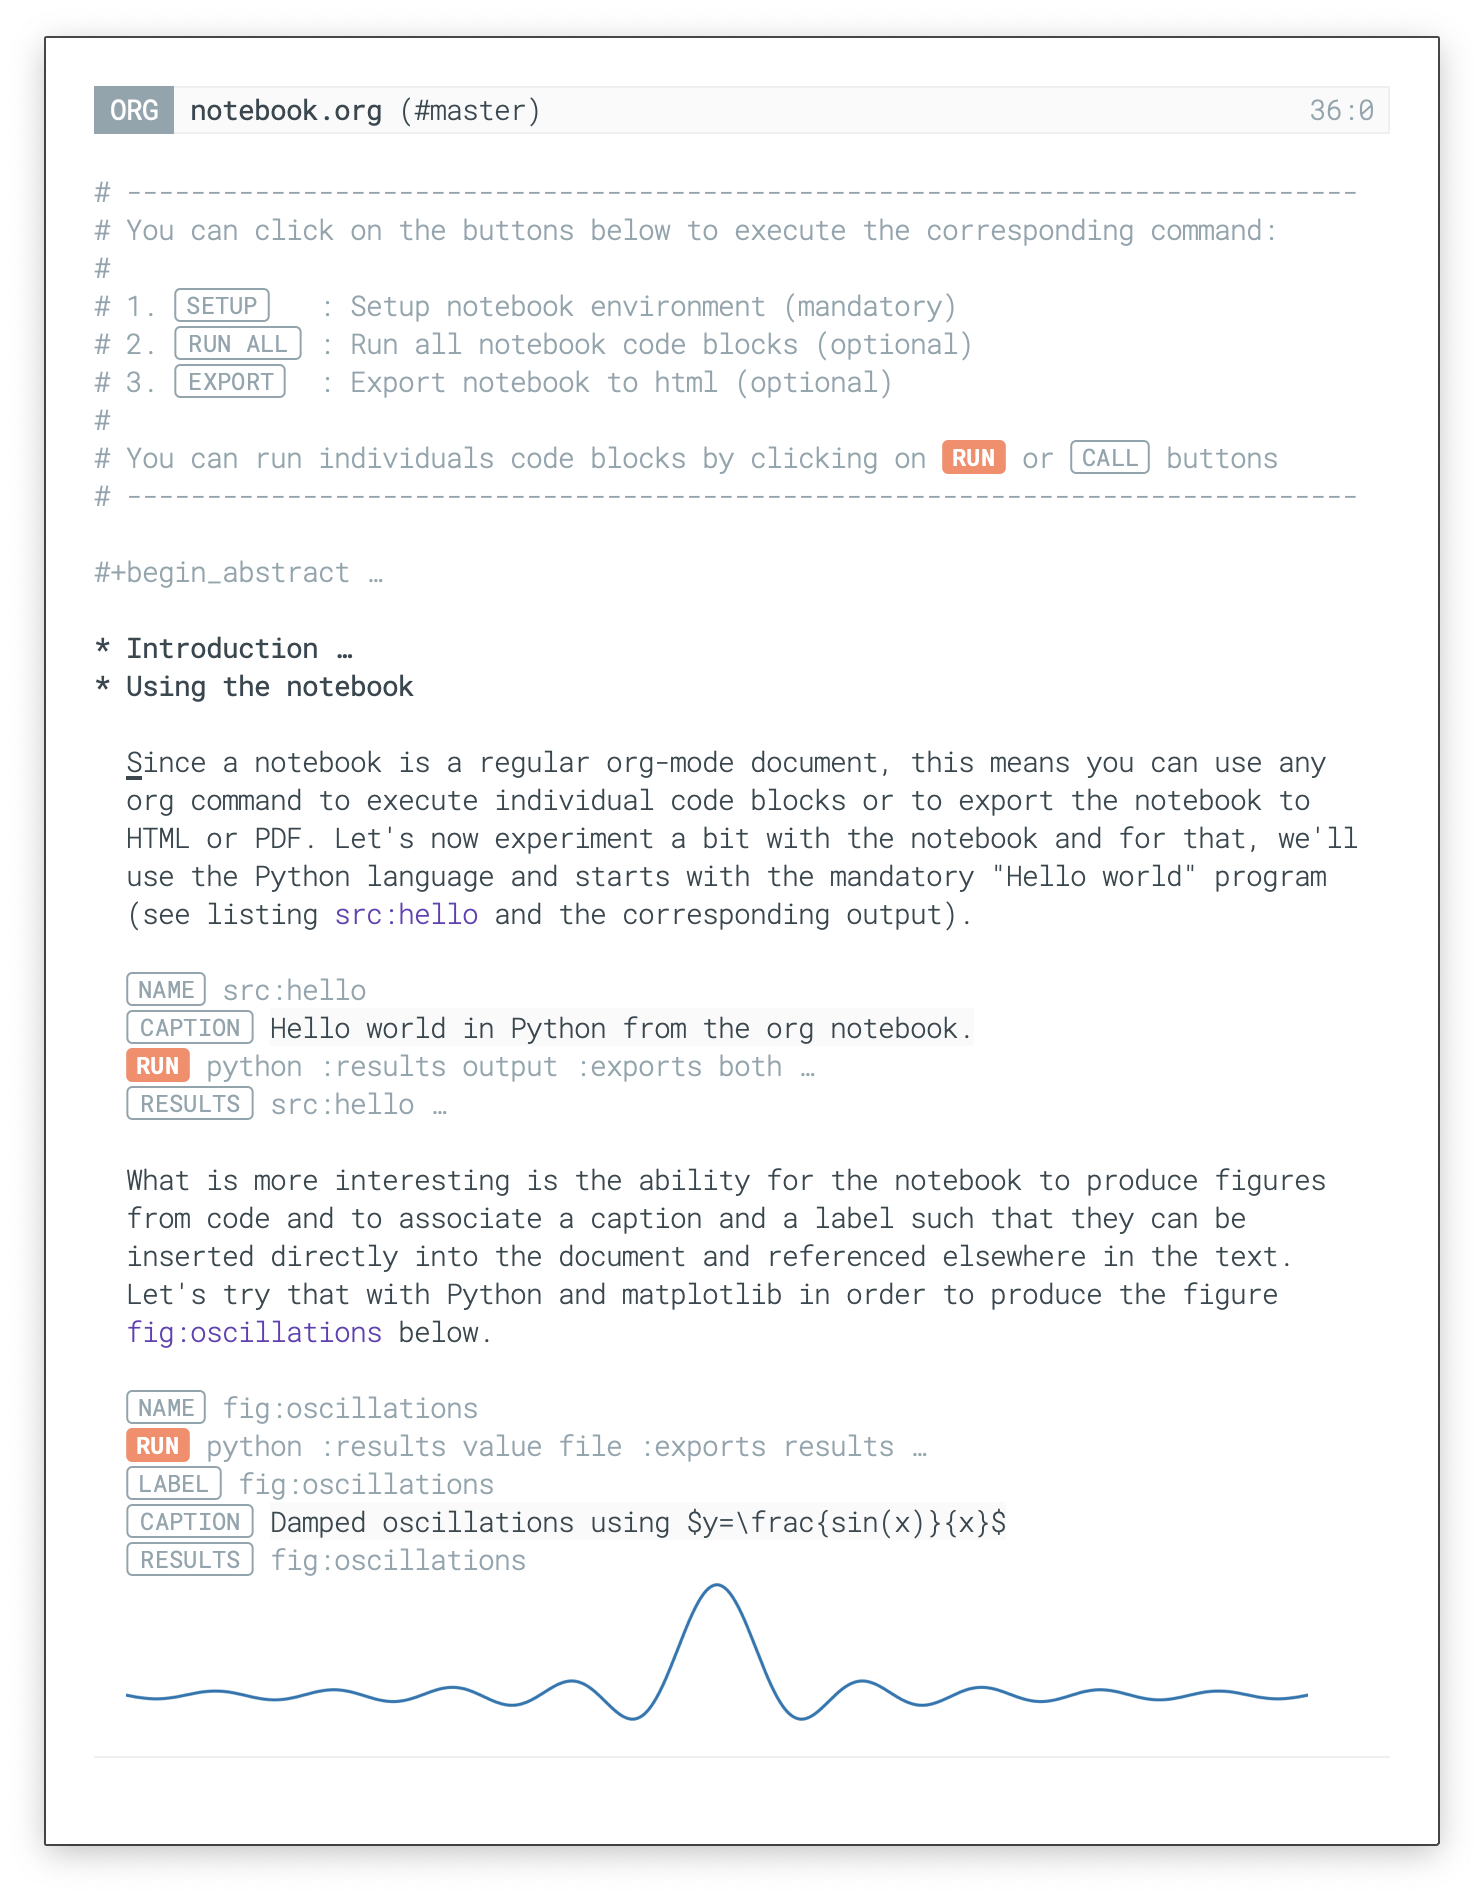
\includegraphics[width=.9\linewidth]{notebook.png}
\caption{\label{fig:teaser}\textbf{The org notebook as rendered inside GNU Emacs.} \href{https://www.gnu.org/software/emacs/}{GNU Emacs} can be hacked such as to offer a clean and legible interface for the notebook that is is actually a regular \href{https://orgmode.org/}{org-mode} document. This means a user can write and run the notebook fully inside Emacs, without the need to install any extra tools (but the different languages used inside the notebook, of course). In other words, everything is handled by Emacs. The advantage of the org notebook is that you can have block of code in any language and even mix them. This actually what have been used to display the enviroment in the abstract box, mixing Emacs lisp and Python. The theme used in the screenshot is \href{https://github.com/rougier/nano-theme}{NΛNO Theme} (available on \href{https://elpa.gnu.org/}{ELPA}) and the font is \href{https://fonts.google.com/specimen/Roboto+Mono}{Roboto Mono}. See [cite:@Rougier:2020] for further details.}
\end{figure}
\end{sidefig}

\section*{Using the notebook}
\label{sec:org7f94eec}

Since a notebook is a regular org-mode document, this means you can use any org command to execute individual code blocks or to export the notebook to HTML or PDF. Let's now experiment a bit with the notebook and for that, we'll use the Python language and starts with the mandatory "Hello world" program (see listing \ref{src:hello} and the corresponding output).

\begin{listing}[htbp]
\begin{minted}[frame,linenos=true]{python}
print("Hello world!")
\end{minted}
\caption{\label{src:hello}Hello world in Python from the org notebook.}
\end{listing}
\begin{verbatim}
Hello world!
\end{verbatim}

The inline equivalent would result in: \texttt{Hello world!}

What is more interesting is the ability for the notebook to produce figures from code and to associate a caption and a label such that they can be inserted directly into the document and referenced elsewhere in the text. Let's try that with Python and matplotlib in order to produce the figure \ref{fig:oscillations} below.

\begin{figure}[htbp]
\centering
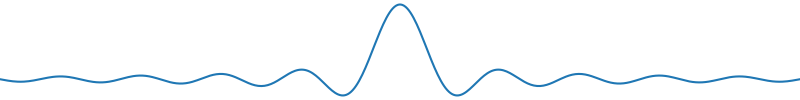
\includegraphics[width=.9\linewidth]{oscillations.png}
\caption{\label{fig:oscillations}Damped oscillations using \(y=\frac{sin(x)}{x}\)}
\end{figure}

From this simple example, you can start experimenting with literate
programming in any language or combinations of languages. For
example, the environment that is declared in the top box of this
document is automatically generated when the document is exported and it mixes code in Python (to get Python version) and code in Emacs lisp (to get Emacs version). Possibilities are infinite.

\section*{References}
\label{sec:orgc37d672}
\end{document}